\subsection{Problem With Using Perplexity in Hyperparameter Search}
In \autoref{subsec:hyperparameters}, the way we found the optimal hyperparameters for the \gls{lda} model is described.
There, it is described that we evaluated the models based on both perplexity and human evaluation.
Human evaluation was necessary because of the way perplexity is calculated for models.

The model that had the lowest perplexity of $202.913$ had the hyperparameters: $(K=15, \alpha =0.01, \eta =0.1)$.
In comparison, the model that was chosen for the experiment had a perplexity of $212.511$ and had the hyperparameters: $(K=30, \alpha =0.1, \eta =0.1)$.
If we used purely perplexity for choosing the hyperparameters for the model, we would have ended up using a model with 15 topics.
Instead we used both perplexity and human evaluation of the models, based on which models had the most humanly understandable topics.
Here we evaluated the models with the lowest perplexities for these K-values: 5, 10, 15, 20, 25, 30, and 35.
We did not look beyond 35, because the perplexity became significantly higher.\todo[inline]{Måske passer noget af dette bedre i gridsearch afsnittet.}
When looking at the most representative words of the first 5 topics in the 15-topic model, as seen in \autoref{fig:15TopicWords}, it is clear that what these topics cover is too wide.

\begin{figure}[h]
	\centering
	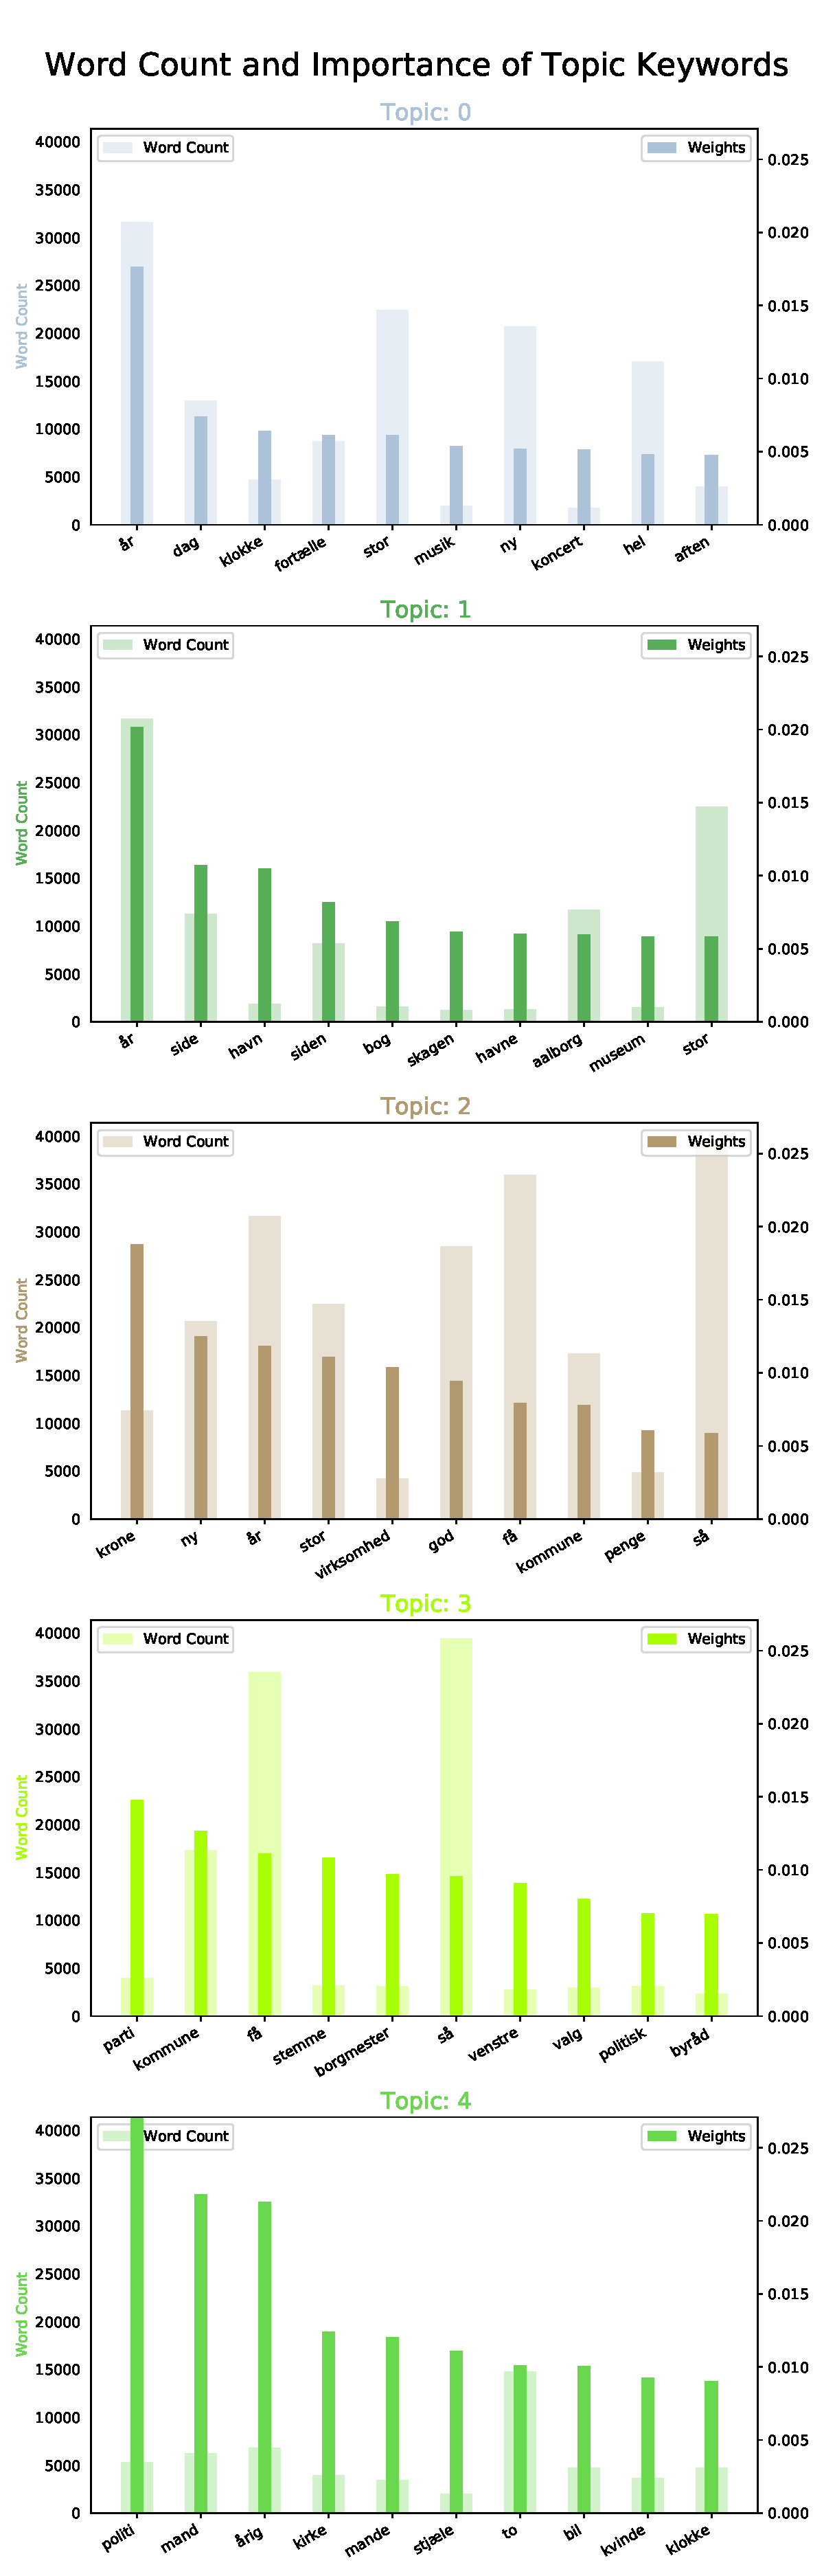
\includegraphics[width=0.45\textwidth]{figures/Word count and importance_corpus2017_document_model(15, 0.01, 0.1)(15, 0.01, 0.1)_topic 0-4.pdf}
	\caption{The first 5 topics from the 15-topic model.
	The most important words for each topic, sorted by the words weight in the topic, are shown.}
	\label{fig:15TopicWords}
\end{figure}

This indicates that the granulaty of the dataset at 15 topics is too low to give humanly understandable topics.
When looking at the most representative words of the first 5 topics in the 30-topic model, as seen in \autoref{fig:30TopicWords}, some more understandable topics can be seen.
Though, it can also be seen that while some topics in the 30-topic model are still difficult to interpret, other topics are much more understandable.

\begin{figure}[h]
	\centering
	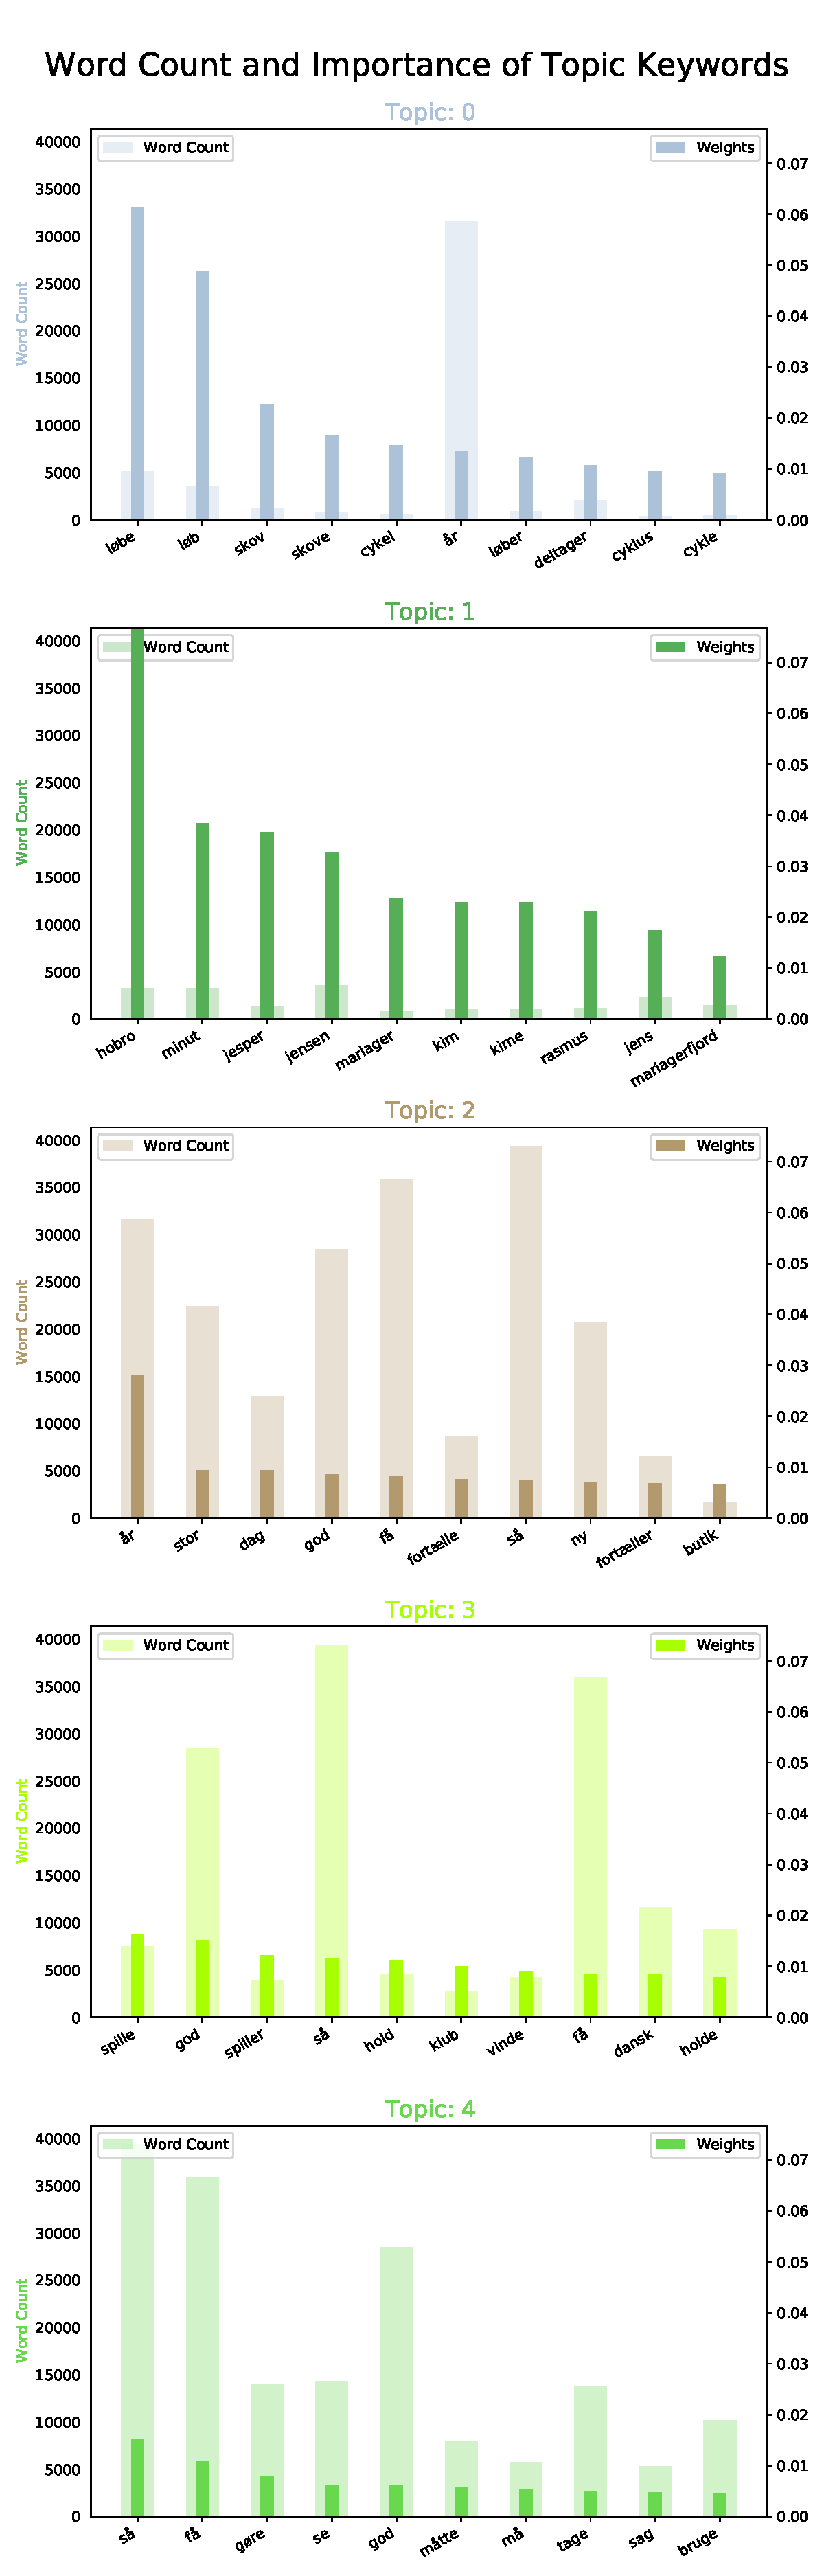
\includegraphics[width=0.45\textwidth]{figures/Word count and importance_corpus2017_final_model(30, 0.1, 0.1)(30, 0.1, 0.1)_topic 0-4.pdf}
	\caption{The first 5 topics from the chosen 30-topic model.
		The most important words for each topic, sorted by the words weight in the topic, are shown.}
	\label{fig:30TopicWords}
\end{figure}

This shows a conflict between using the best perplexity and having a good granularity, which is why perplexity by itself was evaluated to not be enough to choose the hyperparameters for the experiment.
